\documentclass[tikz, varwidth=6in]{standalone}

\newcommand{\FCNB}{
	\begin{tabular}{c|c}
		\multicolumn{2}{c}{} \\\hline
		\, & \,
	\end{tabular}
}

\tikzset{
	fit rounded/.style={
		draw,
		rounded corners,
		inner sep =+ 0pt,
		minimum width = .8cm,
		minimum height = .8cm
	}
}

% arara: pdflatex: { interaction: batchmode }
% arara: latexmk: { clean: partial }
\begin{document}
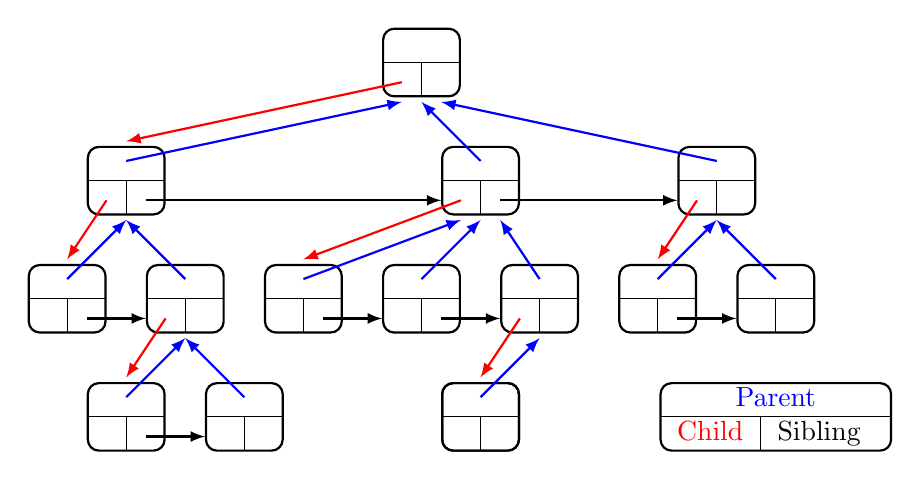
\begin{tikzpicture}[
	level distance=1.5cm,
	level 1/.style={sibling distance=5cm},
	level 2/.style={sibling distance=2.5cm},
	edge from parent/.style={draw,-latex},
	thick
]

\node[fit rounded]  at (4.50,3.0) {\FCNB{}};

\node[fit rounded]  at (0.75,1.5) {\FCNB{}};
\node[fit rounded]  at (5.25,1.5) {\FCNB{}};
\node[fit rounded]  at (8.25,1.5) {\FCNB{}};

\node[fit rounded]  at (0.0,0.0) {\FCNB{}};
\node[fit rounded]  at (1.5,0.0) {\FCNB{}};
\node[fit rounded]  at (3.0,0.0) {\FCNB{}};
\node[fit rounded]  at (4.5,0.0) {\FCNB{}};
\node[fit rounded]  at (6.0,0.0) {\FCNB{}};
\node[fit rounded]  at (7.5,0.0) {\FCNB{}};
\node[fit rounded]  at (9.0,0.0) {\FCNB{}};

\node[fit rounded]  at (0.75,-1.5) {\FCNB{}};
\node[fit rounded]  at (2.25,-1.5) {\FCNB{}};
\node[fit rounded]  at (5.25,-1.5) {\FCNB{}};
\node[fit rounded]  at (5.25,-1.5) {\FCNB{}};

\draw[-latex] (1.00, -1.75) -> (1.75, -1.75);
\draw[-latex] (0.25, -0.25) -> (1.00, -0.25);
\draw[-latex] (3.25, -0.25) -> (4.00, -0.25);
\draw[-latex] (4.75, -0.25) -> (5.50, -0.25);
\draw[-latex] (7.75, -0.25) -> (8.50, -0.25);
\draw[-latex,red] (1.25, -0.25) -> (0.75, -1.00);
\draw[-latex,blue] (0.75, -1.25) -> (1.5, -0.50);
\draw[-latex,blue] (2.25, -1.25) -> (1.5, -0.50);
\draw[-latex,blue] (5.25, -1.25) -> (6, -0.50);
\draw[-latex,red] (5.75, -0.25) -> (5.25, -1.00);

\draw[-latex,red] (0.50, 1.25) -> (0.00, 0.5);
\draw[-latex,blue] (0.00, 0.25) -> (0.75, 1.00);
\draw[-latex,blue] (1.5, 0.25) -> (0.75, 1.00);
\draw[-latex] (1.00, 1.25) -> (4.75, 1.25);

\draw[-latex,red] (5.0, 1.25) -> (3.00, 0.50);
\draw[-latex,blue] (3, 0.25) -> (5.00, 1.00);
\draw[-latex,blue] (4.5, 0.25) -> (5.25, 1.00);
\draw[-latex,blue] (6.0, 0.25) -> (5.50, 1.00);
\draw[-latex] (5.50, 1.25) -> (7.75, 1.25);

\draw[-latex,red] (8.00, 1.25) -> (7.5, 0.50);
\draw[-latex,blue] (7.5, 0.25) -> (8.25, 1.00);
\draw[-latex,blue] (9.0, 0.25) -> (8.25, 1.00);

\draw[-latex,red] (4.25, 2.75) -> (0.75, 2.00);
\draw[-latex,blue] (0.75, 1.75) -> (4.25, 2.50);
\draw[-latex,blue] (5.25, 1.75) -> (4.50, 2.50);
\draw[-latex,blue] (8.25, 1.75) -> (4.75, 2.50);

\node[fit rounded] at (9,-1.5) {
	\begin{tabular}{c|c}
		\multicolumn{2}{c}{\textcolor{blue}{Parent}} \\\hline
		\textcolor{red}{Child} & Sibling \,
	\end{tabular}
};

\end{tikzpicture}
\end{document}
